\documentclass[letterpaper]{article}
\usepackage[utf8]{inputenc}
\usepackage{CJKutf8}
\usepackage{graphicx}

\title{Exercise 1}
\author{Changxuan Li (immoke)}
\date{\today}

\begin{document}
\maketitle

\begin{CJK*}{UTF8}{gbsn}
\section{Introduction}
此次作业完成了使用带Armijo条件的梯度下降法对Rosenbrock函数进行优化,完成对2维和3维函数的测试,本程序均可快速收敛至最小点。
如图~\ref{fig:result}所示,起始点为$(-1,-1)$,本方法经过几次迭代迅速接近全局最小点,并在$(1,1)$点处收敛,与预先分
析结果一致。
\end{CJK*}
\begin{figure}[h]
    \centering
    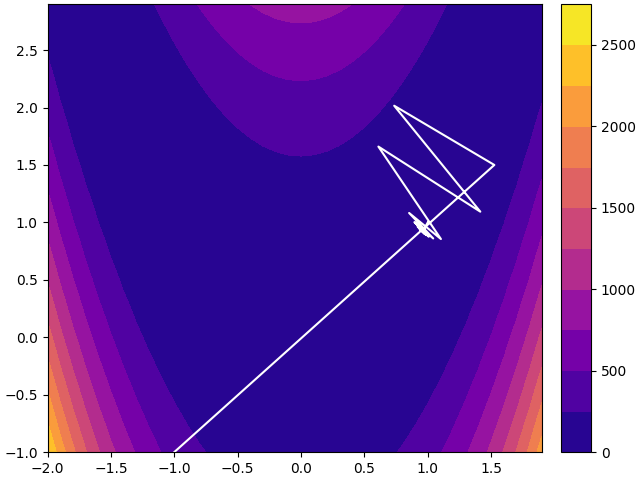
\includegraphics[width=\textwidth]{../media/2D_inexact.png}
    \caption{Steepest gradient descent on Rosenbrock function}
    \label{fig:result}
\end{figure}

\section{Implementation}
\begin{CJK*}{UTF8}{gbsn}
本次作业代码主要分为三个部分:函数及其导数,梯度下降法的实现以及可视化。
\subsection{函数及其导数}
为实现对于N维函数的兼容性,函数数值从1维开始按照函数公式进行累加。
\\\\
\noindent1阶导数由分析法求得,并兼容N维函数。原本希望使用ceres库对函数进行数值求导,但由于该库对变量类型要求比较严格,使用
较为复杂,暂时使用分析法求导,\underline{希望之后课程中也可以分享实践技巧,方便将理论知识运用到项目中。}

\subsection{梯度下降法}
在本部分中,实现了带Armijo条件的梯度下降法。此方法由单独函数实现并通过具有广泛性的梯度下降框架进行调用。在该框架下,可以方便
地调用其他方法。为方便传递优化器所需的函数,定义config结构,通过简单改变名称即可调用其他方法。

\subsection{可视化}
通过pybind11调用matplotlib库进行绘图。Wiki上的Rosenbrock函数图像应该是经过对数标准化,可以继续尝试,绘制出类似的图像。
\end{CJK*}
\section{Discussion}
\begin{CJK*}{UTF8}{gbsn}
本次作业内容难度不大,但是可以通过多实现几种方法进行扩展以及比较,进一步加深对各个方法的理解。之后可以从求导,增加优化方法,
可视化以及速度上进行迭代补充。

\subsection{问题}
1. 测试4维函数时,运行时间较长,梯度的norm在一定时间保持不变,认为可能是由于\underline{学习率过小}导致,请问有无解决办法?
并且希望可以有相应benchmark可以对比验证。(图表待更新)。
\\
2. 希望可以推荐一些优化库以及使用技巧,方便之后在实际项目中使用。
\end{CJK*}
\end{document}